\documentclass[border=2mm]{standalone}
\usepackage{tikz}
\usetikzlibrary{shapes.symbols}

\begin{document}

\if09
correct forbidden sign
forbidden sign
magnifying glass
cloud
    cloud puffs=4
    cloud puff arc=245
    cloud ignores aspect=true
starburst
    starburst points=1
    starburst point height=1cm
    random starburst=1
signal
    signal pointer angle=45
    signal from=west|nowhere|east|north|south
    signal to=west|nowhere|east|north|south
tape
    tape bend top=out and in
    tape bend bottom=out and in|none
    tape bend height=1cm
magnetic tape
    magnetic tape tail extend=0.2cm
    magnetic tape tail=0.24cm
    
\fi


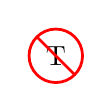
\begin{tikzpicture}[every node/.style={name=a,yshift=-1cm,line width=1pt,draw=red,fill=white,draw}]


\path node[correct forbidden sign] at(0,0){T};
;





\end{tikzpicture}







 
 
\end{document}